% Project report: ROUGH OUTLINE ONLY.
% Bullets are notes for the author, not final prose. Numbers come from
% filter_project/HANDOFF.md and results/*.csv (10M-key base DB) and should be
% re-checked against the notebook before they go into the final text.
%
% Template: PVLDB style, which is acmart in sigconf mode without ACM
% metadata. acmart ships with TeX Live, so this compiles on Overleaf as is.
\documentclass[sigconf,nonacm]{acmart}

\usepackage{booktabs}
\usepackage{xcolor}

\graphicspath{{figures/}{../figures/}}

% Author notes, visible in the PDF. Delete before submission.
\newcommand{\todo}[1]{\textcolor{red}{\textbf{[TODO: #1]}}}
% Box standing in for a figure that does not exist yet.
\newcommand{\placeholder}[1]{\fbox{\parbox[c][3.2cm][c]{0.92\columnwidth}{\centering\small #1}}}

\begin{document}

\title{Bloom, Ribbon or Cuckoo? An Experimental Comparison of SST Filters in RocksDB}

\author{Lucas Caudill}
\affiliation{%
  \institution{University of Massachusetts Boston}
  \city{Boston}
  \country{USA}}

\begin{abstract}
\todo{Write last. 4--6 sentences: problem (point lookups in LSM trees probe
one filter per sorted run), what we did (Bloom, Ribbon and a new cuckoo filter
implemented in RocksDB, compared on one shared DB), main findings (I/O-bound:
FPR per bit decides, Ribbon wins at equal memory; in-memory: \todo{E6
result}; build cost: \todo{E8 result}; cuckoo only pays off above
$\approx$12 bits/key), takeaway for practitioners.}
\end{abstract}

\maketitle

% PVLDB papers print a "PVLDB Reference Format" block here. Not needed for a
% course report.

%======================================================================
\section{Introduction}
\label{sec:intro}

\begin{itemize}
  \item LSM trees (RocksDB, LevelDB, Cassandra) trade read cost for write
    throughput: a point lookup may visit every sorted run
    \cite{oneil1996lsm,dong2021rocksdb}.
  \item Per-SST filters avoid most of those I/Os for runs that do not hold the
    key. Absent-key lookups are common (insert-if-not-exists, joins,
    deduplication).
  \item The design question (course option P4, ``which structure?''): which
    filter should an LSM use, and under what conditions? Filters differ in FPR
    per bit, query CPU and construction cost.
  \item Contributions:
    \begin{enumerate}
      \item A cuckoo filter \cite{fan2014cuckoo} implemented as a RocksDB
        \texttt{FilterPolicy} (whole and partitioned filters, batched
        \texttt{MultiGet}).
      \item A methodology that compares filters on \emph{one} physical DB:
        rebuild only the filter blocks per configuration and verify that the
        LSM shape is identical.
      \item Experiments in two regimes (I/O-bound and in-memory), at equal
        \emph{real} bits/key, plus filter construction cost.
      \item A simple cost model that explains I/O-bound absent-key throughput
        ($R^2 = 0.991$).
    \end{enumerate}
  \item One-paragraph summary of findings. \todo{after E6--E8}
\end{itemize}

%======================================================================
\section{Background}
\label{sec:background}

\subsection{Point lookups in LSM trees}
\begin{itemize}
  \item Leveled compaction, one filter per SST, filter and index blocks in the
    block cache (\texttt{cache\_index\_and\_filter\_blocks}).
  \item Cost of an absent-key lookup $\approx$ (filters probed) $\times$ FPR
    $\times$ (cost of a data block read). The last term depends on whether
    the block is cached: this is what separates our two regimes.
  \item Related: Monkey reallocates bits across levels \cite{dayan2017monkey};
    RocksDB's \texttt{bloom\_before\_level} hybrid uses cheap-to-build Bloom
    for young levels.
\end{itemize}

\subsection{Filters compared}
Table~\ref{tab:filters} summarizes the three filters.
\begin{itemize}
  \item \textbf{Bloom} \cite{bloom1970}: RocksDB's cache-local variant
    (all $k$ probes in one 64-byte line) \cite{putze2009cacheefficient}.
    FPR $\approx (1-e^{-k/b})^k$, slightly worse than textbook at high $b$.
  \item \textbf{Ribbon} \cite{dillinger2021ribbon}: solves a linear system
    over GF(2); $\approx$30\% less space than Bloom at equal FPR, but
    $\approx$4$\times$ slower to build. RocksDB's \texttt{bits\_per\_key} for
    Ribbon is Bloom-equivalent (ribbon-14.3 $\approx$ 10 real bits/key).
  \item \textbf{Cuckoo} \cite{fan2014cuckoo}: $f$-bit fingerprints in
    4-slot buckets, two candidate buckets per key. FPR $\approx 8\alpha/2^f$
    at load $\alpha$, real size $f/\alpha$ bits/key. Beats Bloom only at
    high bits/key. Also mention Xor filters \cite{graf2020xor} as a related
    static design (not evaluated).
\end{itemize}

\begin{table}[t]
  \caption{Filters compared. \todo{fill in construction cost and query CPU
  from filter\_bench (E7)}}
  \label{tab:filters}
  \small
  \begin{tabular}{lccc}
    \toprule
    & Bloom & Ribbon & Cuckoo \\
    \midrule
    FPR at 10 real bits/key & 0.90\% & \todo{} & 1.40\% \\
    Build (ns/key) & $\approx$35 & $\approx$130 & $\approx$52 \\
    Query, in cache (ns) & 6--8 & \todo{} & 23--27 \\
    Build memory & \todo{} & \todo{} & $\approx$12.5 B/key \\
    \bottomrule
  \end{tabular}
\end{table}

%======================================================================
\section{A Cuckoo Filter for RocksDB}
\label{sec:cuckoo}

\begin{itemize}
  \item Interface: \texttt{FilterPolicy} / \texttt{FilterBitsBuilder} /
    \texttt{FilterBitsReader}; string form \texttt{cuckoofilter:<bits>};
    own compatibility name (cannot read Bloom/Ribbon filters or vice versa).
  \item Sizing: $f = \lfloor 0.95\, b \rfloor$ clamped to $[4,32]$, table
    sized so the real size tracks the budget $b$, load capped at 95\%.
  \item Alternate bucket $(H(fp) - i) \bmod n$: an involution for any $n$,
    so table size need not be a power of two (saves space vs.\ the original
    XOR scheme).
  \item Static build at \texttt{Finish()}: random-walk eviction, 500 kicks,
    grow table by 1/16 on failure. In practice every build succeeded on the
    first attempt (incl.\ $f=4$, 20M keys).
  \item Bit-packed fingerprints plus 8-byte trailer; malformed filter
    $\Rightarrow$ ``may match'' (safe).
  \item Testing: unit tests, end-to-end DB test (Get, MultiGet, partitioned,
    reopen under Bloom), independent code review.
  \item Limitations (be upfront): construction memory not charged to the
    block cache; weaker construction-corruption check than built-in filters;
    no stress-test coverage; lookups not tuned (no SIMD).
\end{itemize}

\subsection{Space efficiency and integer fingerprints}
\label{sec:cuckoo-sizing}
\begin{itemize}
  \item Fingerprints are whole bits, so FPR vs.\ bits/key is a sawtooth:
    the efficient points are $b = f/0.95$ (full load). Between them, extra
    space only lowers $\alpha$.
  \item Under a fixed budget, $f = \lfloor 0.95 b\rfloor$ is already the best
    choice; rounding $f$ up exceeds the budget.
  \item Quantify (Figure~\ref{fig:cuckoo-sawtooth}): at 10 bits/key,
    $f=9$, $\alpha=0.9$, model 1.41\%, measured 1.40\%. A hypothetical
    fractional $f=9.5$ at $\alpha=0.95$ gives $\approx$1.05\%. So integer
    rounding explains about half of the gap to Bloom-10 (0.90\%); the rest
    is intrinsic to cuckoo at low bits/key.
  \item Possible fix (not implemented / \todo{if implemented}):
    semi-sorted buckets \cite{fan2014cuckoo} save $\approx$1 bit per entry;
    model predicts $\approx$0.70\% at 10 bits/key, better than Bloom, at
    the cost of slower lookups.
\end{itemize}

\begin{figure}[t]
  \centering
  \placeholder{NEW (E7): cuckoo measured FPR vs.\ real bits/key, fine sweep
  6--24 in 0.25 steps; overlay model $8\alpha/2^f$, fractional-$f$ ideal,
  Bloom measured.}
  \caption{Cuckoo FPR sawtooth from integer fingerprint widths.}
  \label{fig:cuckoo-sawtooth}
\end{figure}

%======================================================================
\section{Methodology}
\label{sec:method}

\subsection{One database for every filter}
\begin{itemize}
  \item Instructor constraint: all experiments on the same DB.
  \item Load once (\texttt{filluniquerandom}, seed 42), then per filter: copy
    the base, run \texttt{rebuildfilters} (single-file
    \texttt{CompactFiles} into the same level, no trivial moves), verify
    per-level shape (files, entries, data blocks, data bytes) against the
    base. Only filter blocks differ.
  \item Reads run \texttt{-readonly}; the harness checks the DB directory is
    unchanged and the found fraction matches the workload.
  \item Missing keys must sort \emph{between} existing keys (append one
    byte), otherwise SST key ranges exclude them before any filter is
    probed. Explain why widening \texttt{-num} is wrong.
\end{itemize}

\subsection{Setup}
\begin{itemize}
  \item Hardware: 24$\times$ Xeon Silver 4214R @ 2.4\,GHz, shared machine.
    \todo{disk model, RAM, OS, RocksDB v11.8.1 + patches}
  \item DB (I/O-bound regime): 10M keys, 64\,B keys, 440\,B values,
    4.89\,GiB, 5{,}237 SSTs in L1--L8, size ratio 2, 1\,MB SSTs, 4\,KB
    blocks, no compression, direct I/O. $\approx$4.5 filters probed per
    absent-key lookup.
  \item DB (in-memory regime): 1M keys, $\approx$0.5\,GB, same LSM settings,
    cache larger than the DB. \todo{filters probed per lookup at 1M keys}
  \item Measurement: warm-up pass, \texttt{resetstats}, measured pass;
    3 repeats; error bars $\pm$1 std. Median CV $\approx$1.5\%.
  \item Metrics: throughput, p50/p99 latency, FPR (from
    \texttt{bloom\_filter\_useful} / \texttt{full\_positive}), data block
    reads per lookup, cache misses by block type.
\end{itemize}

%======================================================================
\section{Results}
\label{sec:results}

\subsection{FPR and memory (E1)}
\begin{itemize}
  \item FPR vs.\ bits/key for all three filters
    (Figure~\ref{fig:e1-fpr}). Add the theoretical lower bound $2^{-b}$.
  \item Cuckoo matches its model; Bloom drifts above the textbook model at
    high $b$; cuckoo/Bloom crossover $\approx$12 bits/key, as predicted by
    $1.44x = (x+3)/0.95$.
\end{itemize}

\begin{figure}[t]
  \centering
  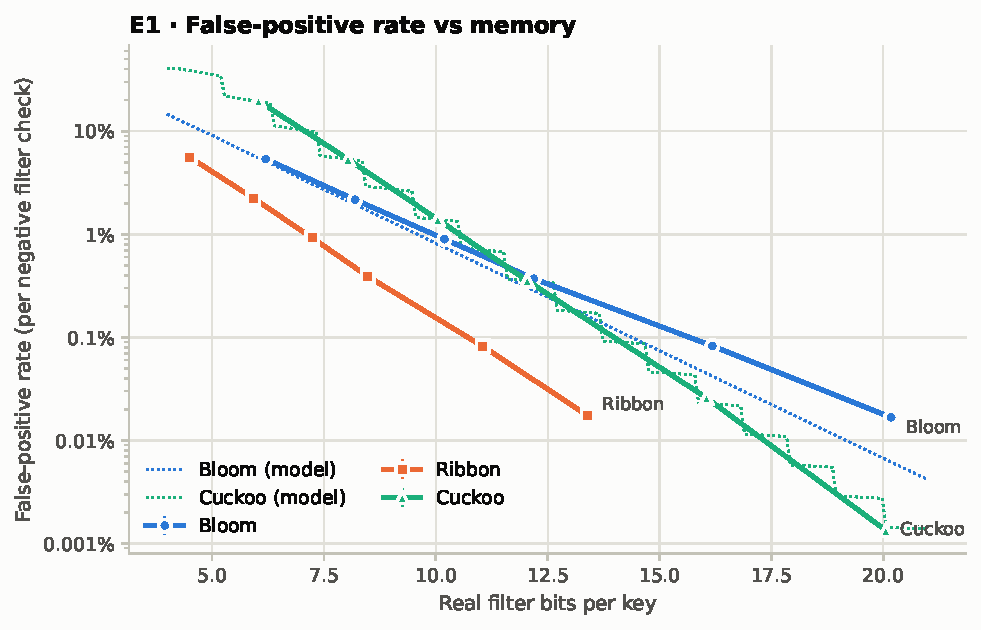
\includegraphics[width=\columnwidth]{e1_fpr_vs_bits}
  \caption{FPR vs.\ bits/key (E1). \todo{redraw against \emph{real}
  bits/key, add $2^{-b}$ bound}}
  \label{fig:e1-fpr}
\end{figure}

\subsection{Equal real bits/key and construction cost (E7)}
\begin{itemize}
  \item Instructor request: compare all filters at the same \emph{real}
    memory (6, 8, 10, 12, 16, 20 bits/key), Ribbon configs calibrated.
  \item FPR and construction ns/key at each point; build memory.
  \item \todo{results: who wins where; cost of Ribbon's space savings in
    build time}
\end{itemize}

\begin{figure}[t]
  \centering
  \placeholder{NEW (E7): (a) FPR vs.\ real bits/key, (b) construction
  ns/key vs.\ real bits/key, one hue per filter.}
  \caption{Filters at equal real memory.}
  \label{fig:e7}
\end{figure}

\subsection{I/O-bound regime: FPR decides (E1--E3)}
\begin{itemize}
  \item Absent keys: no filter $\approx$3.1K lookups/s; filters
    30--65$\times$ higher. Existing keys: $\approx$2.5$\times$ with any
    filter, filters within a few \%. p99 drops $\approx$10$\times$ once
    $4.5\times\mathrm{FPR} < 1\%$ (Figure~\ref{fig:e1-tput}).
  \item Cost model: time per absent lookup $= 5.7\,\mu s + 86\,\mu s \times$
    (data block reads per lookup), $R^2 = 0.991$ across all filters;
    predicts no-filter case within 11\% (Figure~\ref{fig:e1-model}).
    Filter CPU cost is invisible here.
  \item Memory pressure (E2): Ribbon-14.3 (Bloom-10's memory) is
    1.6--2.0$\times$ Bloom-10 for absent keys at every cache size; for
    existing keys, metadata misses at 32--64\,MB, Ribbon-10 halves filter
    misses at 64\,MB (Figure~\ref{fig:e2}).
  \item Absent fraction (E3): filters climb steeply near 100\% absent;
    16 bits/key $\approx$2$\times$ 10 bits/key only near 100\%.
  \item Caveat to state: this regime favors Ribbon (false positives cost a
    disk read).
\end{itemize}

\begin{figure}[t]
  \centering
  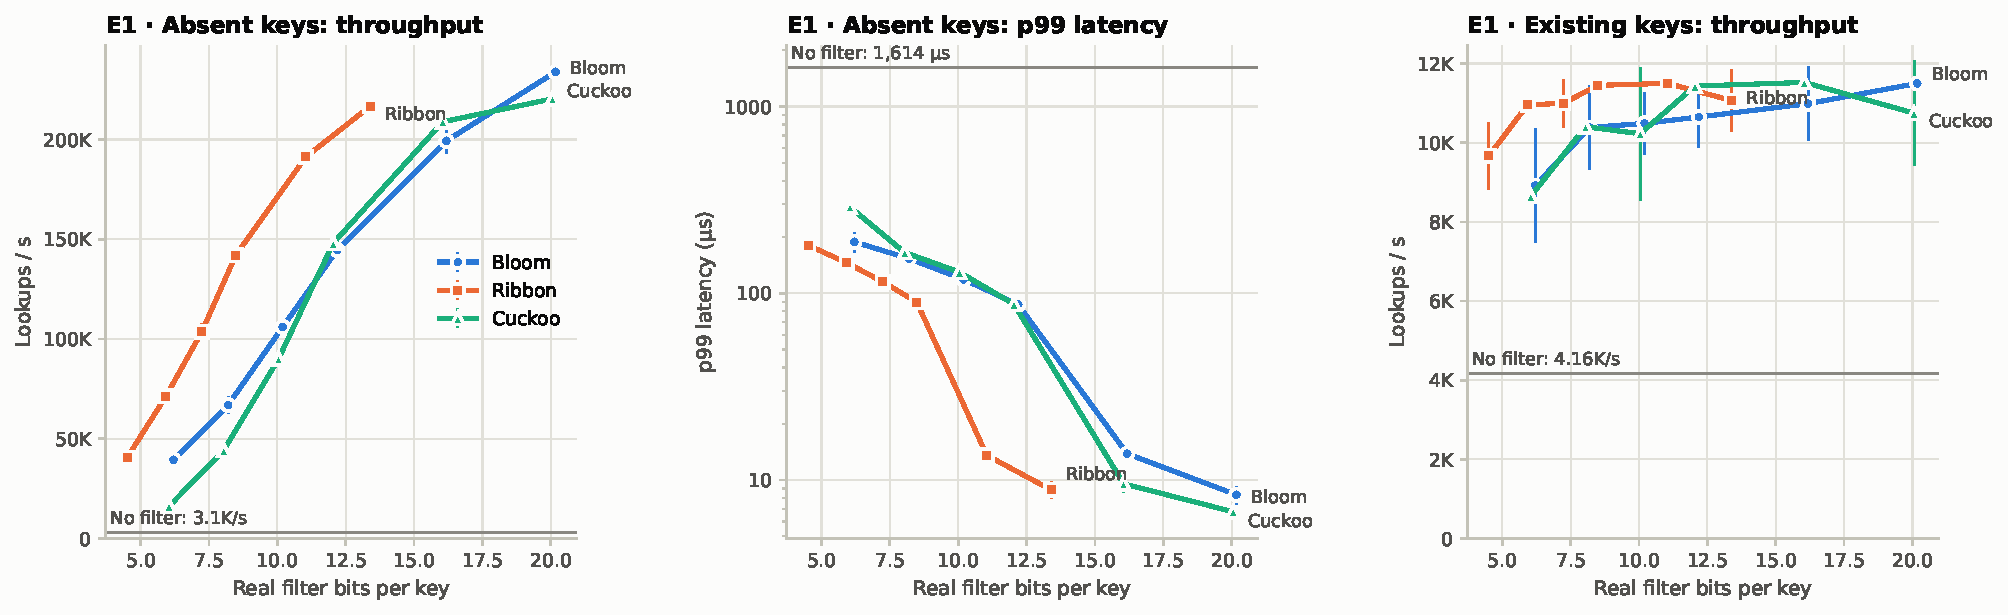
\includegraphics[width=\columnwidth]{e1_throughput_latency}
  \caption{Throughput and tail latency vs.\ bits/key (E1).}
  \label{fig:e1-tput}
\end{figure}

\begin{figure}[t]
  \centering
  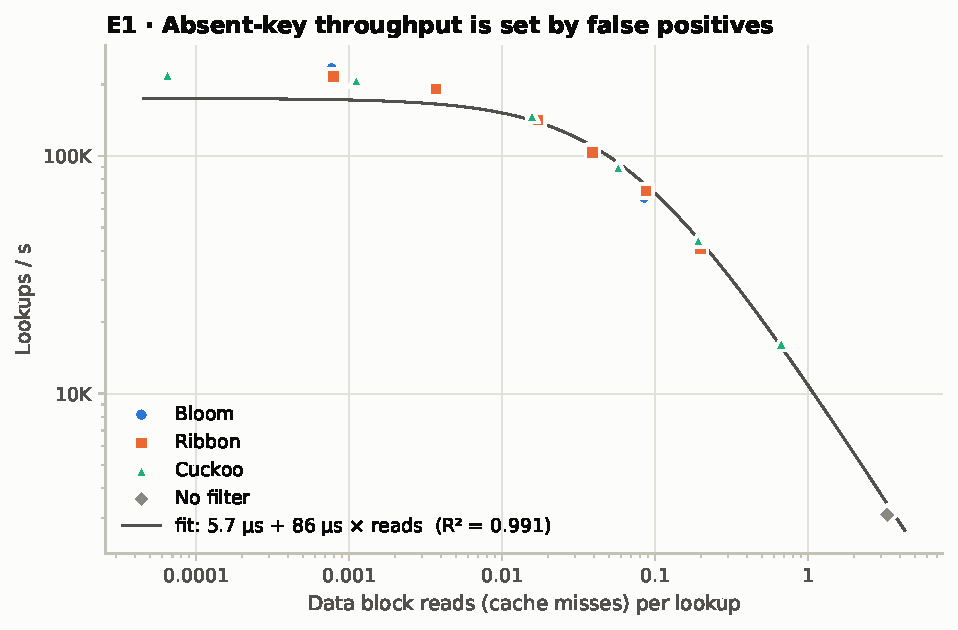
\includegraphics[width=\columnwidth]{e1_false_positives_explain_throughput}
  \caption{Data block reads per lookup explain absent-key throughput.}
  \label{fig:e1-model}
\end{figure}

\begin{figure}[t]
  \centering
  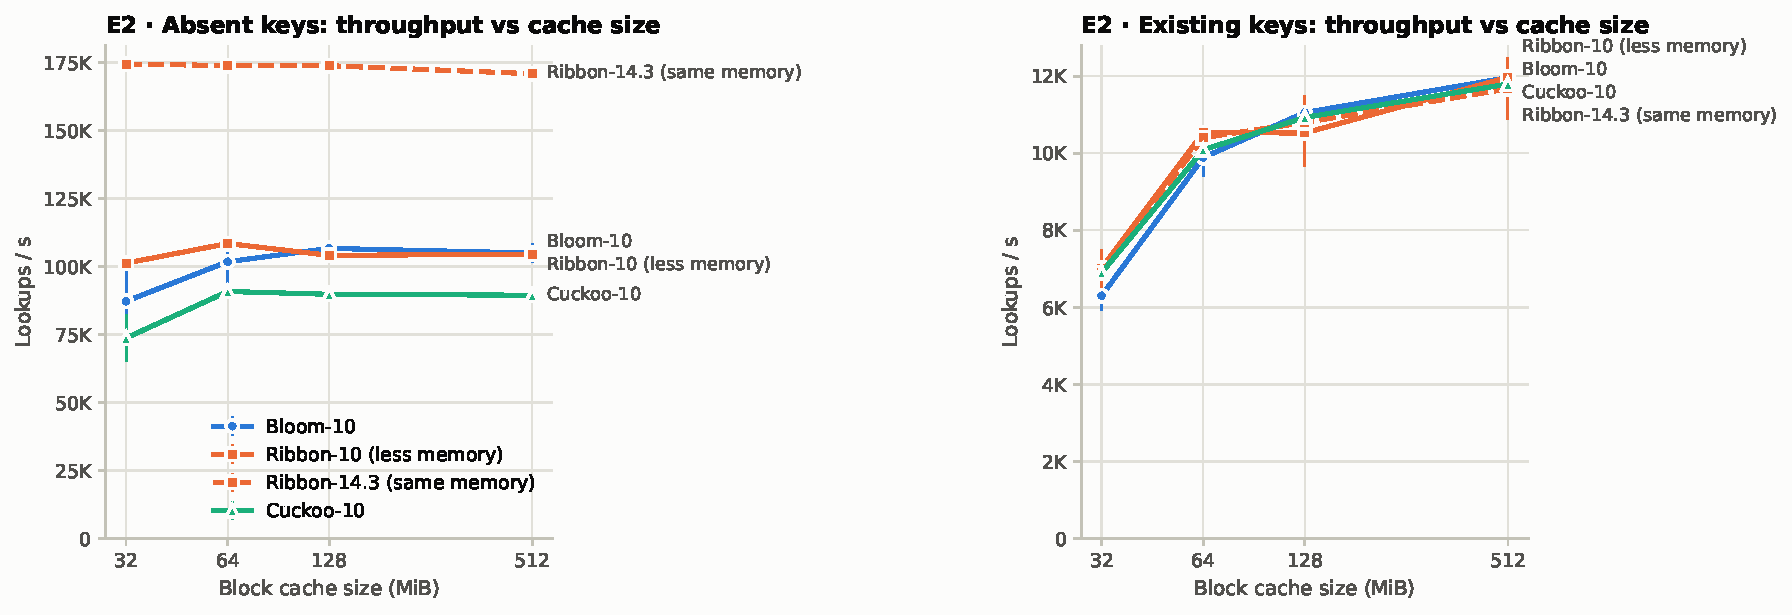
\includegraphics[width=\columnwidth]{e2_throughput_vs_cache}
  \caption{Throughput vs.\ cache size (E2). Possibly also
  \texttt{e2\_cache\_misses\_by\_block\_type}.}
  \label{fig:e2}
\end{figure}

\subsection{In-memory regime: query CPU matters (E6)}
\begin{itemize}
  \item Instructor request: 1M-key DB, cache $>$ DB, workloads
    \texttt{empty} and \texttt{mixed-0.5}, bloom-10, ribbon-14.3,
    cuckoo-10. Warm-up touches every block.
  \item Hypothesis: false positives now cost a cached block lookup, so
    Bloom's cheaper query wins; cuckoo's slower lookup (23--27 vs.\ 6--8 ns)
    becomes visible.
  \item \todo{results; data block reads per lookup should be $\approx$0
    from disk; thread scaling if run}
\end{itemize}

\begin{figure}[t]
  \centering
  \placeholder{NEW (E6): throughput for empty and mixed-0.5, three filters,
  1M keys, cache $>$ DB.}
  \caption{In-memory regime.}
  \label{fig:e6}
\end{figure}

\subsection{Build cost during ingestion (E8, optional)}
\begin{itemize}
  \item \texttt{fillrandom} with compactions per filter (same seed); report
    \texttt{compaction.times.cpu\_micros}, \texttt{db.flush.micros},
    \texttt{stall.micros}; Ribbon with \texttt{bloom\_before\_level} 0 and
    $-1$.
  \item Note: \texttt{rebuildfilters} time ($\approx$155\,s for every
    filter) is dominated by rewriting data, so it does not measure filter
    construction.
  \item \todo{results}
\end{itemize}

\subsection{Skew (E4)}
\begin{itemize}
  \item Throughput rises via data-block caching (data miss ratio
    99\%$\to$44\%); FPR flat; filters within $\approx$6\%. Baseline for
    hotness-aware filters such as ElasticBF.
  \item Optional figure (\texttt{e4\_skew}) or one sentence.
\end{itemize}

% E5 (threads) has a warm-up confound: warm-up is per thread, so more threads
% warm the cache more. Either rerun with constant total warm-up or leave it
% out / mention only "no filter-dependent scaling bottleneck".

%======================================================================
\section{Discussion}
\label{sec:discussion}
\begin{itemize}
  \item Practitioner guidance: which filter when (disk-resident vs.\
    in-memory data, build budget, bits/key). \todo{table or decision list
    after E6--E8}
  \item Chucky \cite{dayan2021chucky}: one global succinct cuckoo filter
    across the LSM. Cannot be expressed through RocksDB's per-SST
    \texttt{FilterPolicy}; discuss what it would change (one probe instead
    of $\approx$4.5).
  \item ElasticBF \cite{li2019elasticbf}: hotness-aware, per-file multiple
    Bloom units. E4 is its baseline. Not implemented.
  \item Threats to validity: shared server (noise), one tree shape (size
    ratio 2, not RocksDB defaults), fixed key/value sizes, untuned cuckoo
    lookups, small DB checks fewer filters per lookup.
\end{itemize}

%======================================================================
\section{Related Work}
\label{sec:related}
\begin{itemize}
  \item Filter designs: Bloom, cache-local Bloom, cuckoo, Xor, Ribbon
    \cite{bloom1970,putze2009cacheefficient,fan2014cuckoo,graf2020xor,dillinger2021ribbon}.
  \item Filters in LSMs: Monkey, Chucky, ElasticBF
    \cite{dayan2017monkey,dayan2021chucky,li2019elasticbf}.
  \item Experimental LSM studies, e.g.\ \cite{sarkar2021compaction}.
\end{itemize}

%======================================================================
\section{Conclusion}
\label{sec:conclusion}
\begin{itemize}
  \item \todo{2--3 sentences once E6--E8 are in.}
  \item Artifact: code and harness at \todo{repo URL / branch}.
\end{itemize}

\bibliographystyle{ACM-Reference-Format}
\bibliography{references}

\end{document}
